\documentclass[11pt]{article}

\usepackage[margin=1in]{geometry}
\usepackage{amsmath}
\usepackage{amssymb}
\usepackage{graphicx}

\emergencystretch=1em

\title{705.641.81: Homework 2}
\author{David Carrillo}
\date{}

\begin{document}
\maketitle

\section{Concepts, intuitions and big picture}

\begin{enumerate}
  \item An $n$-th order Markov assumption throws away everything before the previous $n-1$ words, so it
        cannot represent any dependency longer than that window. Several distinct failures:
        \begin{itemize}
          \item \textbf{Long-distance agreement.} In ``the \emph{keys} to the cabinet \emph{are} on the
                table,'' the verb agrees with \emph{keys}, four words back. A trigram model conditions on
                ``the cabinet'' and will happily prefer the singular \emph{is}.
          \item \textbf{Recursive syntax.} Nested clauses and matched delimiters (parentheses, quotation
                marks, \texttt{if}/\texttt{then}) can be arbitrarily deep. No fixed window can track
                whether a bracket opened 40 tokens ago is still unclosed, because the required memory grows
                with the input.
          \item \textbf{Coreference and discourse.} Resolving \emph{she} or \emph{the company} depends on
                which entity was introduced earlier, often in a previous sentence, which the window has
                already discarded.

          \item \textbf{Scope-bearing operators.} A negation, modal, or quantifier can flip the
                licensing of a word far downstream, past the window.
        \end{itemize}
        The Module 1 lecture on perplexity makes the same point when it notes that count-based models
        ``cannot deal with long range sequences.''

  \item Two things rescue them. First, most of the predictive signal in language really is local: the
        immediately preceding words fix the part of speech and usually the syntactic head, which sharply
        constrains what can come next. Second, language is heavily Zipfian and formulaic, so a small number
        of frequent local patterns account for most tokens, and collocations like ``New York'' or ``in order
        to'' are captured exactly by a short window.

        The grammatical information in the previous word or two is mostly \emph{local syntactic}
        information: part-of-speech transition probabilities (a determiner is followed by a noun or
        adjective, not a finite verb), agreement with an adjacent head, subcategorization of the immediately
        preceding preposition or auxiliary, and morphological continuation within a sub-word sequence. What
        they do not capture is anything requiring structure over the whole sentence. The lecture's own
        numbers show both sides: on Wall Street Journal text perplexity falls from roughly 1000 for a
        unigram model to 170 for a bigram and 109 for a trigram, so almost all of the gain comes from the
        first one or two words of context, and then the curve saturates because sparsity sets in.

  \item They are the same quantity on different scales. Cross-entropy is the average negative log
        probability the model assigns to the held-out tokens,
        \[
          H = -\frac{1}{N}\sum_{i=1}^{N} \log_2 P(w_i \mid w_{<i}),
        \]
        and perplexity is that exponentiated in the same base, $\mathrm{PPL} = 2^{H}$. Because $2^x$ is
        strictly increasing, minimizing cross-entropy loss and minimizing perplexity are the same
        optimization problem, and the training objective for a language model is exactly the metric it is
        evaluated on. The exponentiation buys interpretability: cross-entropy is in bits per token, while
        perplexity is an effective branching factor, the number of equally likely choices the model is
        effectively deciding among. A perplexity of 5 means the model narrowed a large vocabulary down to
        about five candidates, and the lower bound of 1 corresponds to $H = 0$, a model that assigns
        probability 1 to the correct token every time.

  \item If the model is uniform over the vocabulary then $P(w \mid \cdot) = 1/|V|$ for every token, so
        every term of the sum is $-\log(1/|V|) = \log|V|$ and
        \[
          H = \log |V|, \qquad \mathrm{PPL} = b^{\,\log_b |V|} = |V|.
        \]
        A uniform-random model has perplexity exactly $|V|$, which is the natural baseline: it is confused
        among all $|V|$ words and has learned nothing.
        \begin{center}
        \begin{tabular}{|l|r|r|r|}
          \hline
          $|V|$ & Perplexity & Cross-entropy (bits) & Cross-entropy (nats) \\
          \hline
          2000  & 2000  & $\log_2 2000 = 10.966$  & $\ln 2000 = 7.601$ \\
          10000 & 10000 & $\log_2 10000 = 13.288$ & $\ln 10000 = 9.210$ \\
          \hline
        \end{tabular}
        \end{center}
        I give both bases because the lecture defines $\mathrm{PPL} = 2^H$ in bits while Homework 1 stated
        that $\log$ means the natural logarithm; the perplexity is $|V|$ either way, since the base of the
        logarithm and the base of the exponential cancel.

  \item Reasons for the recent wave of neural networks taking off:
        \begin{itemize}
          \item[{[X]}] We have access to a lot more computational power.
          \item[{[\ ]}] Neural Networks are a brand new field.
          \item[{[X]}] We have access to a lot more data.
          \item[{[X]}] There has been significant improvements in benchmarks in speech recognition and NLP.
        \end{itemize}


  \item What does a neuron compute?
        \begin{itemize}
          \item[{[\ ]}] A neuron computes an activation function followed by a linear function
                ($z = Wx + b$).
          \item[{[X]}] A neuron computes a linear function ($z = Wx + b$) followed by an activation
                function.
          \item[{[\ ]}] A neuron computes a function $g$ that scales the input $x$ linearly ($Wx + b$).
          \item[{[\ ]}] A neuron computes the mean of all features before applying the output to an
                activation function.
        \end{itemize}


  \item What is the point of applying a Softmax function to the logits of a sequence classification model?
        \begin{itemize}
          \item[{[\ ]}] It softens the logits so that they're more reliable.
          \item[{[\ ]}] It applies a lower and upper bound so that they're understandable.
          \item[{[X]}] The total sum of the output is then 1, resulting in a possible probabilistic
                interpretation.
        \end{itemize}

\end{enumerate}

\section{Linear Algebra Recap}

\subsection{Gradients}

Let $f(x,y,z) = x^2 y + \sin(z + 6y)$.

\begin{enumerate}
  \item Treating the other two variables as constants each time and applying the chain rule to the sine,
        \[
          \frac{\partial f}{\partial x} = 2xy, \qquad
          \frac{\partial f}{\partial y} = x^2 + 6\cos(z + 6y), \qquad
          \frac{\partial f}{\partial z} = \cos(z + 6y).
        \]
        The factor 6 in $\partial f/\partial y$ is the derivative of the inner function $z + 6y$ with
        respect to $y$.

  \item Stacking the three partials gives the gradient as a vector,
        \[
          \nabla f(\theta) =
          \begin{bmatrix}
            2xy \\ x^2 + 6\cos(z+6y) \\ \cos(z+6y)
          \end{bmatrix}.
        \]
        At $\theta = [3, \pi/2, 0]^\top$ the inner argument is $z + 6y = 0 + 3\pi$, and
        $\cos(3\pi) = -1$, so
        \[
          \nabla f([3,\pi/2,0]^\top) =
          \begin{bmatrix} 2(3)(\pi/2) \\ 9 + 6(-1) \\ -1 \end{bmatrix}
          = \begin{bmatrix} 3\pi \\ 3 \\ -1 \end{bmatrix}
          \approx \begin{bmatrix} 9.4248 \\ 3 \\ -1 \end{bmatrix}.
        \]
\end{enumerate}

\subsection{Gradients of vectors}

Throughout, $\mathbf{x}, \mathbf{c} \in \mathbb{R}^n$ and $\mathbf{A} \in \mathbb{R}^{n \times n}$, and I
use numerator layout as the problem specifies. The shape rule is that differentiating an output of
dimension $m$ by an input of dimension $n$ gives an $m \times n$ object, so a scalar-valued function gives
a $1 \times n$ row vector and a vector-valued function gives an $n \times n$ matrix.

\begin{itemize}
  \item $\dfrac{\partial}{\partial \mathbf{x}}(\mathbf{x}^\top \mathbf{c}) = \mathbf{c}^\top$.

        The output is a scalar, so the derivative is a $1 \times n$ row vector whose $j$-th entry is
        $\partial(\mathbf{x}^\top\mathbf{c})/\partial x_j$. Writing the product as a sum,
        $\mathbf{x}^\top\mathbf{c} = \sum_{i=1}^{n} x_i c_i$. Only the $i = j$ term involves $x_j$, so
        \[
          \frac{\partial}{\partial x_j} \sum_{i=1}^{n} x_i c_i = c_j .
        \]
        Arranging these $n$ entries in a row gives
        $[c_1, \ldots, c_n] = \mathbf{c}^\top$.

  \item $\dfrac{\partial}{\partial \mathbf{x}}\left(\|\mathbf{x}\|_2^2\right) = 2\mathbf{x}^\top$.

        Again scalar output, so a $1 \times n$ row vector. Since
        $\|\mathbf{x}\|_2^2 = \mathbf{x}^\top\mathbf{x} = \sum_{i=1}^{n} x_i^2$, the $j$-th entry is
        \[
          \frac{\partial}{\partial x_j} \sum_{i=1}^{n} x_i^2 = 2x_j ,
        \]
        and stacking into a row gives $2[x_1, \ldots, x_n] = 2\mathbf{x}^\top$.

  \item $\dfrac{\partial}{\partial \mathbf{x}}(\mathbf{A}\mathbf{x}) = \mathbf{A}$.

        Here the output $\mathbf{A}\mathbf{x}$ is a vector in $\mathbb{R}^n$, so the derivative is an
        $n \times n$ matrix, the Jacobian, whose $(i,j)$ entry is $\partial(\mathbf{A}\mathbf{x})_i /
        \partial x_j$. The $i$-th output component is
        $(\mathbf{A}\mathbf{x})_i = \sum_{k=1}^{n} A_{ik} x_k$, and only $k = j$ contributes, so
        \[
          \frac{\partial}{\partial x_j} \sum_{k=1}^{n} A_{ik} x_k = A_{ij} .
        \]
        The entry in row $i$, column $j$ of the derivative is $A_{ij}$, which is precisely $\mathbf{A}$.

  \item $\dfrac{\partial}{\partial \mathbf{x}}(\mathbf{x}^\top \mathbf{A}\mathbf{x})
        = \mathbf{x}^\top(\mathbf{A} + \mathbf{A}^\top)$.

        Scalar output, so a $1 \times n$ row vector. Expanding the quadratic form as a double sum,
        $\mathbf{x}^\top \mathbf{A}\mathbf{x} = \sum_{i}\sum_{k} x_i A_{ik} x_k$, the variable $x_j$ appears
        in two families of terms: those with $i = j$ and those with $k = j$. Differentiating each,
        \[
          \frac{\partial}{\partial x_j} \sum_{i}\sum_{k} x_i A_{ik} x_k
          = \sum_{k} A_{jk} x_k + \sum_{i} x_i A_{ij}
          = (\mathbf{A}\mathbf{x})_j + (\mathbf{A}^\top \mathbf{x})_j
          = \big((\mathbf{A} + \mathbf{A}^\top)\mathbf{x}\big)_j .
        \]
        (The $i = k = j$ term is counted once in each sum, which correctly produces $2A_{jj}x_j$.) Stacking
        the entries into a row vector and transposing,
        $\big((\mathbf{A}+\mathbf{A}^\top)\mathbf{x}\big)^\top
        = \mathbf{x}^\top(\mathbf{A}+\mathbf{A}^\top)$, using the symmetry of
        $\mathbf{A}+\mathbf{A}^\top$. When $\mathbf{A}$ is itself symmetric this collapses to
        $2\mathbf{x}^\top\mathbf{A}$.
\end{itemize}

\subsection{Jacobian}

\begin{enumerate}
  \item For $\mathbf{f}(\boldsymbol{\theta}) = [\sin(x_1x_2x_3),\ \cos(x_2+x_3),\
        \exp(-\tfrac{1}{2}x_3^2)]^\top$, the Jacobian is the $3 \times 3$ matrix
        $J_{ij} = \partial f_i / \partial x_j$:
        \[
          J(\boldsymbol{\theta}) =
          \begin{bmatrix}
            x_2x_3\cos(x_1x_2x_3) & x_1x_3\cos(x_1x_2x_3) & x_1x_2\cos(x_1x_2x_3) \\
            0 & -\sin(x_2+x_3) & -\sin(x_2+x_3) \\
            0 & 0 & -x_3\exp(-\tfrac{1}{2}x_3^2)
          \end{bmatrix}.
        \]
        The zeros are structural: $f_2$ does not depend on $x_1$, and $f_3$ depends only on $x_3$.

  \item At $\boldsymbol{\theta} = [1, \pi, 0]^\top$ we have $x_1x_2x_3 = 0$ so $\cos(0) = 1$, giving the
        first row $[x_2x_3, x_1x_3, x_1x_2] = [0, 0, \pi]$. For the second row $x_2 + x_3 = \pi$ and
        $-\sin(\pi) = 0$. For the third, $-x_3\exp(0) = 0$. Therefore
        \[
          J([1,\pi,0]^\top) =
          \begin{bmatrix}
            0 & 0 & \pi \\
            0 & 0 & 0 \\
            0 & 0 & 0
          \end{bmatrix}.
        \]

\end{enumerate}

\section{$n$-gram Language Models}

\subsection{A toy $n$-gram language model}

\begin{enumerate}
  \item Counting over the six training sentences gives the token counts
        \texttt{BOS}: 6, \texttt{EOS}: 6, \texttt{who}: 5, \texttt{framed}: 4, \texttt{roger}: 4,
        \texttt{rabbit}: 3, \texttt{the}: 1, for a total of $N = 29$ tokens.

        $P(\texttt{rabbit})$ is a unigram estimate, count over total:
        \[
          P(\texttt{rabbit}) = \frac{\text{count}(\texttt{rabbit})}{N} = \frac{3}{29} \approx 0.1034 .
        \]
        This counts \texttt{BOS} and \texttt{EOS} as tokens, which is consistent with the problem listing
        both in $V$. If instead only the five content words are treated as emittable, the denominator is 17
        and the estimate is $3/17 \approx 0.1765$.

        $P(\texttt{rabbit}\mid\texttt{roger})$ is a bigram estimate. The bigrams beginning with
        \texttt{roger} are \texttt{roger rabbit} twice (sentences 3 and 4), \texttt{roger EOS} once
        (sentence 2), and \texttt{roger framed} once (sentence 5), so
        $\text{count}(\texttt{roger}) = 4$ and
        \[
          P(\texttt{rabbit}\mid\texttt{roger})
          = \frac{\text{count}(\texttt{roger}\ \texttt{rabbit})}{\text{count}(\texttt{roger})}
          = \frac{2}{4} = \frac{1}{2} = 0.5 .
        \]

        $P(\texttt{EOS}\mid\texttt{rabbit})$: \texttt{rabbit} occurs 3 times and is followed by
        \texttt{EOS} every time, so
        \[
          P(\texttt{EOS}\mid\texttt{rabbit})
          = \frac{\text{count}(\texttt{rabbit}\ \texttt{EOS})}{\text{count}(\texttt{rabbit})}
          = \frac{3}{3} = 1 .
        \]


  \item The number of possible $n$-grams, $|V|^n$, grows exponentially in $n$ while the corpus stays
        finite, so most $n$-grams are never observed and maximum likelihood assigns them probability
        exactly zero. That is fatal in practice: one zero makes a whole test sentence's probability zero
        and its perplexity infinite. The surviving estimates are also unreliable, since a denominator of 1
        or 2 gives a very high variance estimate. Smoothing redistributes mass onto unseen $n$-grams so no
        estimate is exactly zero; Section 6 measures how severe this is on real data.
\end{enumerate}

\section{Challenges of linear classifiers of sentences}

\begin{enumerate}
  \item With $\mathrm{repr}(s) = \sum_{w \in s} v_w$ and $f(s;\theta) = \theta \cdot \mathrm{repr}(s)$, the
        representation of a two-word phrase is just the sum of its two word vectors, and $f$ is linear in
        that sum. So
        \[
          f(\texttt{not good};\theta) = \theta\cdot(v_{\texttt{not}} + v_{\texttt{good}})
          = \theta\cdot v_{\texttt{not}} + f(\texttt{good};\theta),
        \]
        and likewise for \texttt{bad}. Substituting into the two desired inequalities:
        \begin{align*}
          f(\texttt{good};\theta) > f(\texttt{not good};\theta)
            &\iff f(\texttt{good};\theta) > \theta\cdot v_{\texttt{not}} + f(\texttt{good};\theta)
            \iff 0 > \theta\cdot v_{\texttt{not}}, \\
          f(\texttt{bad};\theta) < f(\texttt{not bad};\theta)
            &\iff f(\texttt{bad};\theta) < \theta\cdot v_{\texttt{not}} + f(\texttt{bad};\theta)
            \iff 0 < \theta\cdot v_{\texttt{not}} .
        \end{align*}
        The two conditions reduce to $\theta\cdot v_{\texttt{not}} < 0$ and
        $\theta\cdot v_{\texttt{not}} > 0$, which cannot both hold for any $\theta$ and any word
        embeddings. Note what dropped out: the vectors $v_{\texttt{good}}$ and $v_{\texttt{bad}}$ cancel
        entirely, so the model's treatment of \texttt{not} is forced to be a single fixed additive shift in
        the score, identical in every context. Negation, however, has to \emph{reverse} sentiment, which
        means shifting scores down for positive words and up for negative ones. A single additive constant
        cannot do both, which is the inadequacy the question points at.

  \item \textbf{Extra credit.} The same mechanism defeats any intensifier, not just negation. Take
        \texttt{very} and ask for
        \[
          f(\texttt{very good};\theta) > f(\texttt{good};\theta),
          \qquad
          f(\texttt{very bad};\theta) < f(\texttt{bad};\theta),
        \]
        which is the obvious requirement that \texttt{very} should push a positive phrase further positive
        and a negative phrase further negative. Expanding both,
        \[
          \theta\cdot v_{\texttt{very}} + f(\texttt{good};\theta) > f(\texttt{good};\theta)
          \iff \theta\cdot v_{\texttt{very}} > 0,
        \]
        \[
          \theta\cdot v_{\texttt{very}} + f(\texttt{bad};\theta) < f(\texttt{bad};\theta)
          \iff \theta\cdot v_{\texttt{very}} < 0,
        \]
        again a contradiction. The general statement is that for any modifier $m$ and any two words
        $w_1, w_2$, the pair $f(m\,w_1) > f(w_1)$ and $f(m\,w_2) < f(w_2)$ is unsatisfiable, because both
        inequalities collapse onto the sign of the single scalar $\theta\cdot v_m$.

  \item \textbf{Extra credit.} With $f(s;\theta) = \theta\cdot\mathrm{ReLU}(\mathrm{repr}(s))$ the
        cancellation no longer happens, because $\mathrm{ReLU}$ is applied after summing and can zero out
        different coordinates for different phrases. A concrete satisfying assignment in $\mathbb{R}^2$:
        \[
          \theta = \begin{bmatrix} 2 \\ 1\end{bmatrix}, \quad
          v_{\texttt{good}} = \begin{bmatrix} 1 \\ 0\end{bmatrix}, \quad
          v_{\texttt{bad}} = \begin{bmatrix} -1 \\ 0\end{bmatrix}, \quad
          v_{\texttt{not}} = \begin{bmatrix} -1 \\ 1\end{bmatrix}.
        \]
        Evaluating each of the four phrases:
        \begin{center}
        \begin{tabular}{|l|l|l|r|}
          \hline
          Phrase & $\mathrm{repr}(s)$ & $\mathrm{ReLU}(\mathrm{repr}(s))$ & $f(s;\theta)$ \\
          \hline
          \texttt{good}     & $[1,0]^\top$  & $[1,0]^\top$ & 2 \\
          \texttt{not good} & $[0,1]^\top$  & $[0,1]^\top$ & 1 \\
          \texttt{bad}      & $[-1,0]^\top$ & $[0,0]^\top$ & 0 \\
          \texttt{not bad}  & $[-2,1]^\top$ & $[0,1]^\top$ & 1 \\
          \hline
        \end{tabular}
        \end{center}
        Both inequalities hold: $f(\texttt{good}) = 2 > 1 = f(\texttt{not good})$ and
        $f(\texttt{bad}) = 0 < 1 = f(\texttt{not bad})$. The mechanism is that
        $\mathrm{ReLU}$ clips the negative first coordinate of $v_{\texttt{bad}}$ to zero, so adding
        $v_{\texttt{not}}$ has a different effect on \texttt{bad} than on \texttt{good}. With these
        embeddings the general condition is $\theta_1 > \theta_2 > 0$.

  \item A linear model on a bag of embeddings can only ever add a fixed per-word contribution to the score,
        so any word's effect is context independent by construction. Neural networks earn their extra
        complexity because a nonlinearity lets a word's contribution depend on what it is combined with,
        which is the minimum needed to represent composition effects like negation, intensification, and
        sarcasm.
\end{enumerate}

\section{Softmax function}

\begin{enumerate}
  \item Substituting $\mathbf{z} + c$ into the definition, the constant factors out of both the numerator
        and every term of the denominator and cancels:
        \[
          \sigma(\mathbf{z} + c)_i
          = \frac{e^{z_i + c}}{\sum_{j=1}^{K} e^{z_j + c}}
          = \frac{e^{c}\,e^{z_i}}{e^{c}\sum_{j=1}^{K} e^{z_j}}
          = \frac{e^{z_i}}{\sum_{j=1}^{K} e^{z_j}}
          = \sigma(\mathbf{z})_i .
        \]
        This holds for every $i$, so $\sigma(\mathbf{z}) = \sigma(\mathbf{z}+c)$.



  \item The denominator $\sum_j e^{z_j}$ is a single positive constant, the same for every component, so
        softmax rescales all entries by one positive number. Writing $Z = \sum_j e^{z_j} > 0$, for any
        indices $i$ and $k$,
        \[
          z_i > z_k
          \iff e^{z_i} > e^{z_k}
          \iff \frac{e^{z_i}}{Z} > \frac{e^{z_k}}{Z}
          \iff \sigma(\mathbf{z})_i > \sigma(\mathbf{z})_k ,
        \]
        where the first step uses that $\exp$ is strictly increasing and the second that dividing by a
        positive constant preserves order. Softmax is therefore a strictly increasing transformation
        applied coordinatewise, so it preserves the entire ranking and in particular
        $\arg\max_i z_i = \arg\max_i \sigma(\mathbf{z})_i$.

  \item For $K = 2$, divide the numerator and denominator by $e^{z_1}$:
        \[
          \sigma_1([z_1,z_2])
          = \frac{e^{z_1}}{e^{z_1} + e^{z_2}}
          = \frac{1}{1 + e^{z_2 - z_1}}
          = \frac{1}{1 + e^{-(z_1 - z_2)}}
          = S(z_1 - z_2),
        \]
        which is the definition of the sigmoid evaluated at $z_1 - z_2$. So two-class softmax is a
        sigmoid on the single logit \emph{difference}: only the gap between the two scores matters, which is
        the same redundancy that shift invariance describes.

  \item \textbf{Extra credit.} Take the reciprocal of $\sigma(\mathbf{z})_i$ and split off the $j = i$
        term:
        \[
          \frac{1}{\sigma(\mathbf{z})_i}
          = \frac{\sum_{j=1}^{K} e^{z_j}}{e^{z_i}}
          = \sum_{j=1}^{K} e^{-(z_i - z_j)}
          = 1 + \sum_{j \ne i} e^{-(z_i - z_j)} .
        \]
        Set $\alpha_j = e^{-(z_i - z_j)}$, which is positive for every $j$. The hinted inequality
        $\big(1 + \sum_j \alpha_j\big) \le \prod_j (1 + \alpha_j)$ for $\alpha_j \ge 0$ then gives
        \[
          \frac{1}{\sigma(\mathbf{z})_i}
          = 1 + \sum_{j \ne i} \alpha_j
          \le \prod_{j \ne i} (1 + \alpha_j)
          = \prod_{j \ne i} \left(1 + e^{-(z_i - z_j)}\right)
          = \prod_{j \ne i} \frac{1}{S(z_i - z_j)} .
        \]
        Both sides are positive, so taking reciprocals reverses the inequality and yields the claim,
        \[
          \sigma(\mathbf{z})_i \ge \prod_{j \ne i} S(z_i - z_j).
        \]
        The hint itself is just the observation that expanding $\prod_j(1+\alpha_j)$ produces
        $1 + \sum_j \alpha_j$ plus all the higher-order products, each of which is nonnegative. Equality
        therefore holds exactly when there are no higher-order terms, that is when $K = 2$, which matches
        item 3.
\end{enumerate}

\section{Programming}

\subsection*{6.1.4 Visualize the $N$-gram distribution}

\begin{center}
  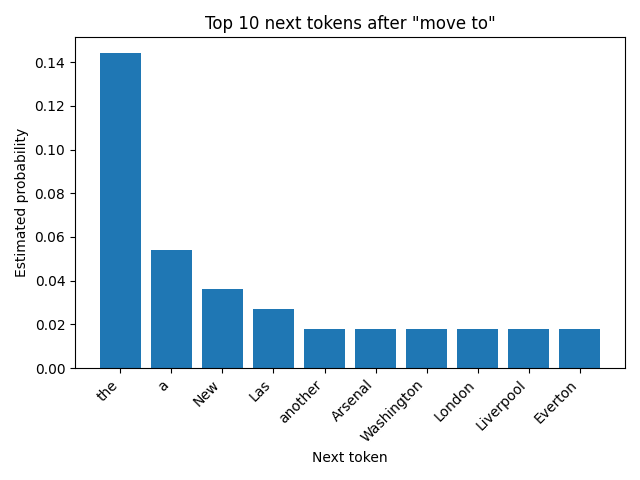
\includegraphics[width=0.62\textwidth]{hw2/ngram_context1.png}
\end{center}
\begin{center}
  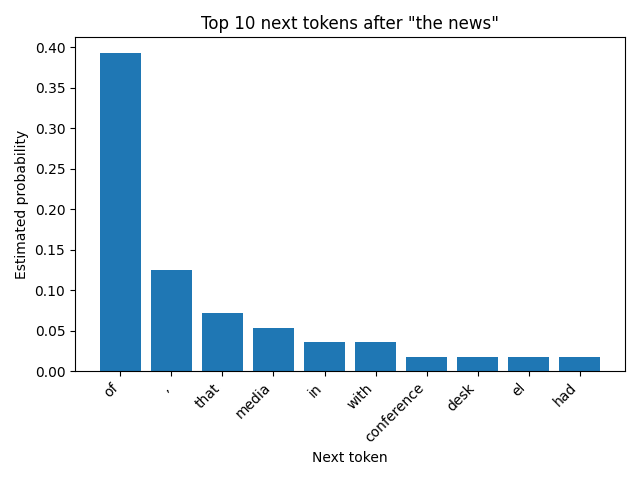
\includegraphics[width=0.62\textwidth]{hw2/ngram_context2.png}
\end{center}

Measured statistics for the two contexts, from the trigram model built on the first $10^5$ WikiText-103
paragraphs:

\begin{center}
\small
\begin{tabular}{|l|r|r|r|r|r|}
  \hline
  Context & count & next tokens & top-1 prob & top-10 mass & singletons \\
  \hline
  \texttt{("move", "to")} & 111 & 80 & 0.144 (\texttt{the}) & 0.369 & 70 of 80 \\
  \texttt{("the", "news")} & 56 & 22 & 0.393 (\texttt{of}) & 0.786 & 16 of 22 \\
  \hline
\end{tabular}
\end{center}

\textbf{Findings.}
The two contexts are peaked very differently: \texttt{"the news"} puts 0.393 on \texttt{of} and 78.6\% of
its mass in the top ten, while \texttt{"move to"} manages only 0.144 and 36.9\%. The difference is
linguistic, since \texttt{"move to"} takes an open class of destinations while \texttt{"the news"} mostly
takes function words. Both plots show a plateau of equal-height bars, which is that open class appearing
once each: 70 of the 80 continuations of \texttt{"move to"} rest on a single observation.

\subsection*{6.1.5 Generation: Sample from the LM}

\begin{center}
\begin{tabular}{|p{0.27\textwidth}|p{0.61\textwidth}|}
  \hline
  Prefix & Greedy completion \\
  \hline
  ``According to the report'' & \emph{According to the report, the first time in the United States, and
  the other hand, the first time in the United States, and the other hand, the first time} \\
  \hline
  ``The president of the association'' & \emph{The president of the association ' s " The One I Love You
  ' re not here to Connacht side of the game ' s " The One I Love You ' re not} \\
  \hline
\end{tabular}
\end{center}

\textbf{Findings.}
Both completions collapse into a loop, and the repetition is inevitable rather than unlucky. Greedy
decoding is deterministic and the trigram context is only two tokens wide, so once generation re-enters a
context it has already visited it must emit the same continuation forever. The second completion also
stitches together locally fluent but unrelated fragments, jumping from a quoted song title to a Connacht
rugby reference, which is what a two-token memory looks like.

\subsection*{6.2.4 Gradient Descent}

\begin{center}
  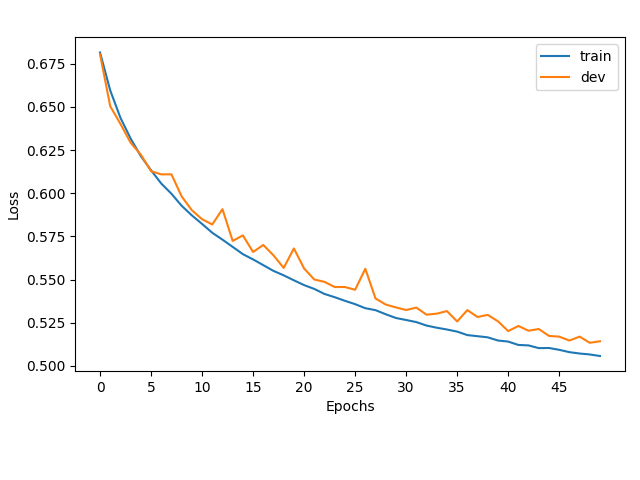
\includegraphics[width=0.62\textwidth]{hw2/gradient_descent_loss.png}
\end{center}

Configuration: \texttt{glove-twitter-50}, batch size 64, learning rate 0.05, 50 epochs, with the softmax,
cross-entropy loss, gradients, and parameter updates all implemented by hand rather than by
\texttt{autograd}.

\begin{center}
\begin{tabular}{|l|r|r|r|r|r|r|}
  \hline
  Epoch & 0 & 10 & 20 & 30 & 40 & 49 \\
  \hline
  Dev loss & 0.6805 & 0.5850 & 0.5564 & 0.5324 & 0.5201 & 0.5142 \\
  Dev acc & 0.5040 & 0.7280 & 0.7360 & 0.7700 & 0.7630 & 0.7600 \\
  \hline
\end{tabular}
\end{center}

Test set: loss 0.5256, accuracy 0.7570. Best dev accuracy 0.7700 at epoch 30; minimum dev loss 0.5134 at
epoch 48.

\textbf{Findings.}
Both curves are still descending over the final ten epochs, with the minimum dev loss at epoch 48, so this
run has not converged. Plain gradient descent at a fixed 0.05 learning rate reaches 0.757 test accuracy
against 0.795 for the Adam version in Homework 1, on identical features and an identical 102-parameter
classifier. The gap is optimizer and budget, not capacity.

\end{document}
